\Dword{tc} is responsible for detector integration
and installation support. 
%The technology for massive noble liquid detectors has developed over the last \num{45} years and the first large \dword{lartpc} was completed in 2010. While multiple \dwords{lartpc} have operated worldwide, the technology is still relatively new and the scale up to \dword{dune} presents challenges. However, the technology is well suited to massive neutrino detectors with millimeter scale resolution on \SI{100}{m} scale detectors and the technical challenges are surmountable.
The \dword{dune} collaboration consists of a large number of
institutions distributed throughout the world. They are supported by a
large number of funding sources and collaborate with a large number of
commercial partners. Groups of institutes within \dword{dune} form
consortia that take complete responsibility for construction of their
system.  \dword{dune} has empowered several consortia (currently nine)
with the responsibility to secure funding and design, fabricate,
assemble, install, commission and operate their components of the
\dword{dune} \dword{fd}. There are three consortia focusing
exclusively on the \dword{spmod}: \dword{apa},
\single \dword{ce} and \single \dword{pds}. There are three
focusing exclusively on the \dword{dpmod}: 
\dword{crp}, \dual \dword{ce} and \dual \dword{pds}. There are
three joint consortia: \dword{hv}, \dword{daq} and \dword{cisc}. Other consortia may
be formed over time as concepts more fully emerge, such as a
\dword{fd} calibration system and various aspects of the \dword{nd}.
\dword{dune} \dword{tc}, under the direction of the
%\dword{dune} 
Technical Coordinator, has responsibility to monitor the
technical aspects of the detector construction, to integrate and
install the \dwords{detmodule} and to deliver the common projects. The
\dword{dune} \dword{tc} organization is shown in Figure~\ref{fig:TC_orgchart}.

\begin{dunefigure}[Organization of \dword{tc}]{fig:TC_orgchart}
  {Organization of \dword{tc}. This organization
 oversees the construction of the \dword{fd}, both \single and
 \dual, and the \dword{nd}.}
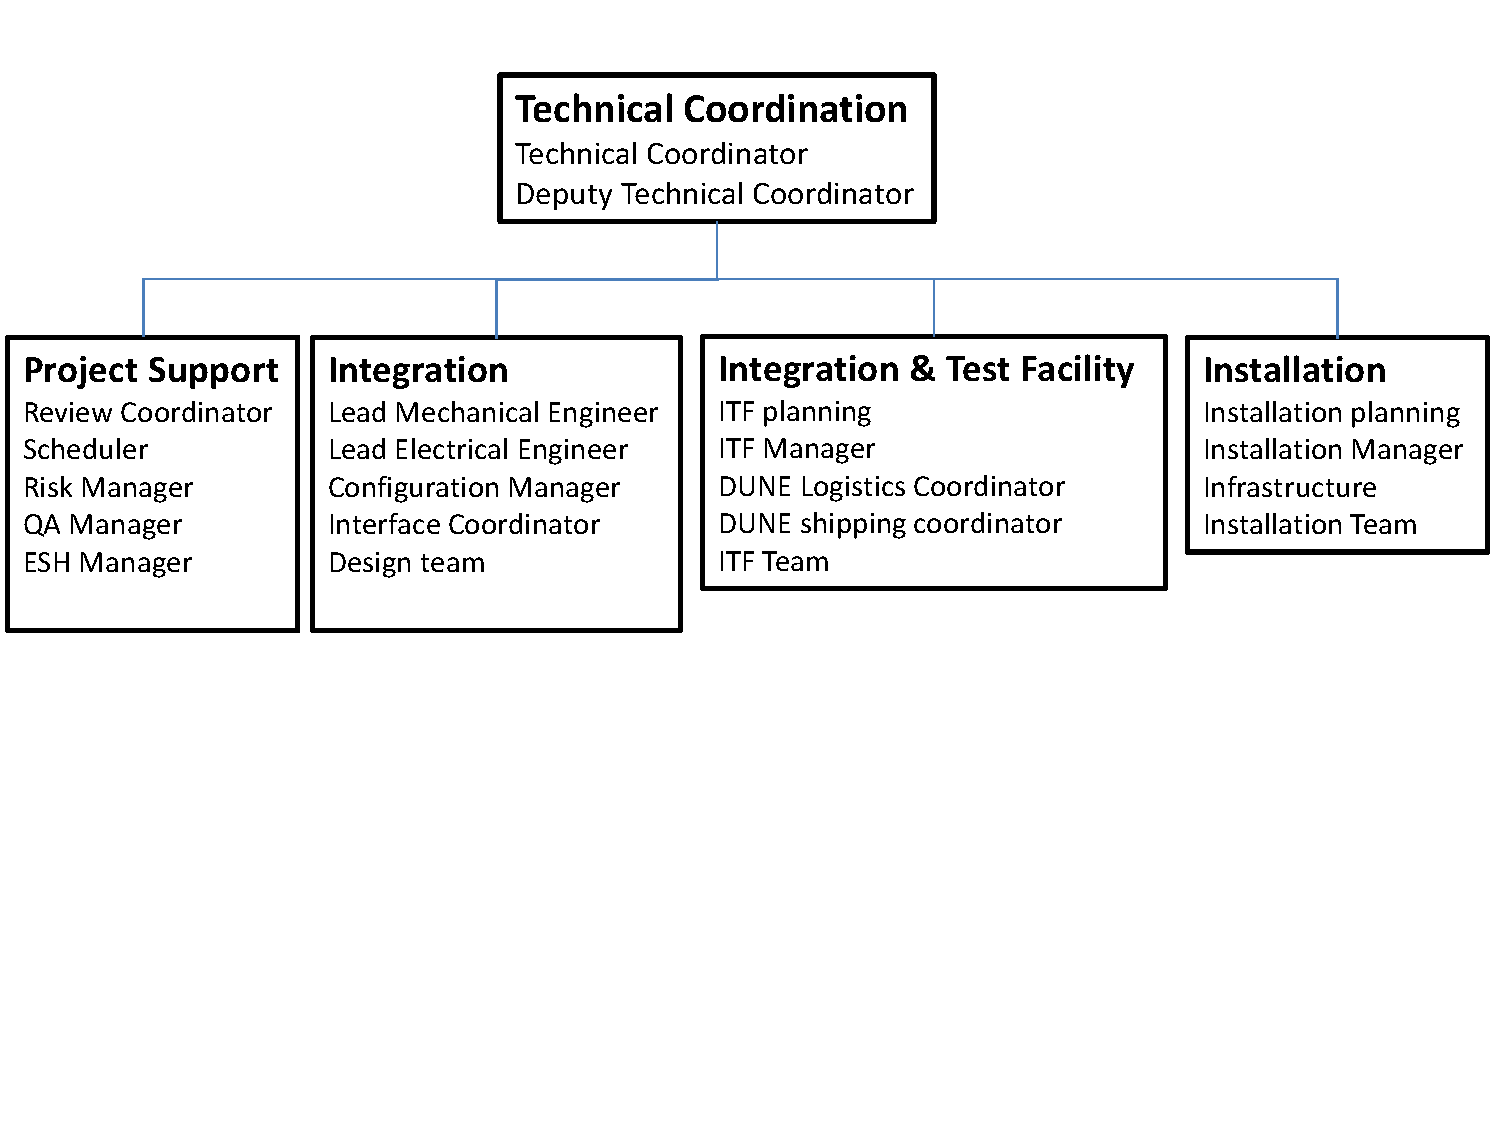
\includegraphics[width=\textwidth]{TP_TC_Org_Chart}
\end{dunefigure}


The \dword{tc} organization staffing will grow over time as the project
advances. \Dword{tc} will provide staffing for teams underground at \surf, at
integration facilities, and at the near site at \fnal, in addition to
the core team distributed among collaborating institutions.

The \dword{dune} Project consists of a \dword{fd} and a
\dword{nd}. The \dword{nd} is at a pre-conceptual state; as the
conceptual design and organization emerges, it will become part of the
\dword{dune} Project. Currently the \dword{dune} Project consists of
the \dword{dune} \dword{fd} consortia and \dword{tc}.  The
\dword{dune} Project is moving towards a \dword{tdr} for
the \dword{fd}, both \single and \dual options, in 2019. It is
expected that a Conceptual Design Report for the \dword{nd} will be
prepared at the same time. 

The \dword{fd} components will be shipped
from the consortia construction sites to the \dword{itf}. 
\Dword{tc} will
evaluate and accept consortia components either at integration
facilities or the installation site and oversee the integration of
components as appropriate. The scope of the \dword{fd} integration
and installation effort is shown graphically in
Figure~\ref{fig:TC_flow}.

\begin{dunefigure}[Flow of components from the consortia to the \dword{fd}.]{fig:TC_flow}
  {Flow of components from the consortia to the \dword{fd}.}
 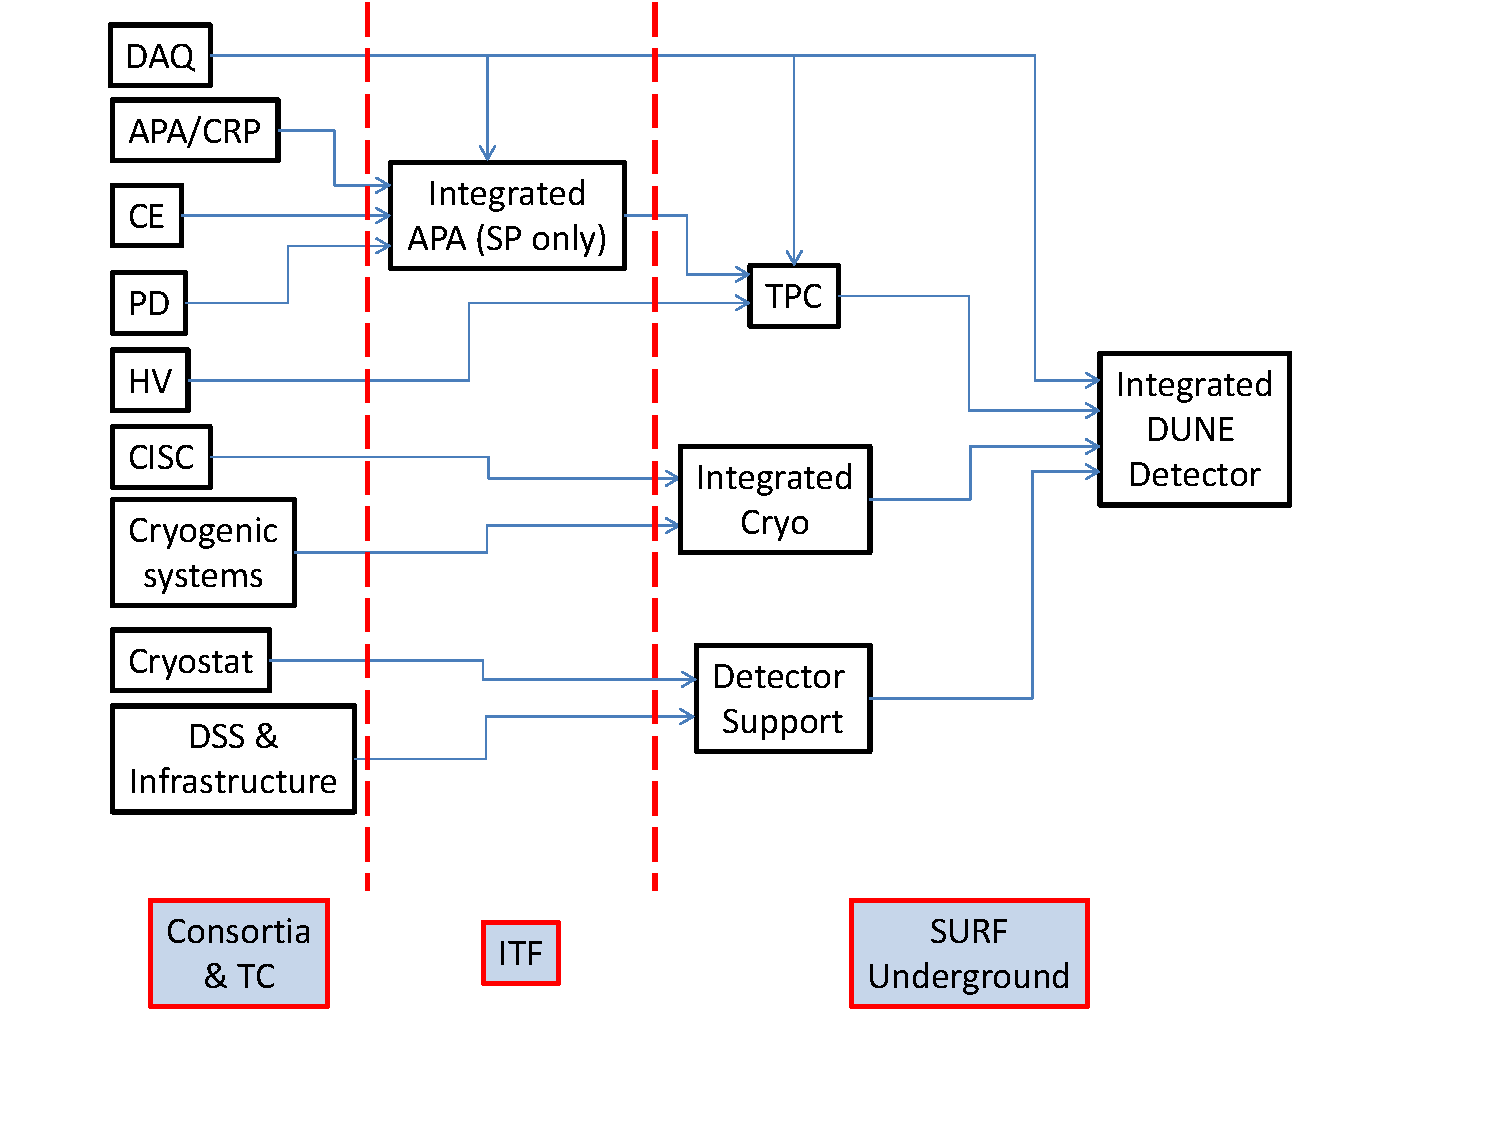
\includegraphics[width=\textwidth]{DUNE_deliverable_flow}
\end{dunefigure}

\Dword{tc} interacts with the consortia via three main areas: project
coordination, integration, and installation.  Construction of the
\dword{dune} \dword{fd} requires careful technical coordination due to
its complexity.  Given the horizontal nature of the consortia
structure and the extensive interdependencies between the systems, a
significant engineering organization is required to deliver
\dword{dune} on schedule and within specifications and funding
constraints.

The responsibilities of \dword{tc} include:
\begin{itemize}
  \item management and delivery of all common projects;
  \item development and monitoring of the consortia interfaces;
  \item configuration control of all interface documents, drawings and envelopes;
  \item installation of detectors at the near and far sites;
  \item logistics for detector integration and installation at the near and far sites;
  \item survey of the detector;
  \item primary interface to \dword{lbnf} for conventional facilities, cryostat and cryogenics;
  \item primary interface to the host laboratory for infrastructure and operations support;
  \item development and tracking of project schedule and milestones;
  \item review of all aspects of the project;
  \item recording and approving all project engineering information, including: documents, drawings and models;
  \item project work breakdown schedules;
  \item project risk register;
  \item \dword{dune} engineering and safety standards, including grounding and shielding;
  \item monitoring of all consortia design and construction progress;
  \item \dword{qa} and all \dword{qa} related studies and documents;
  \item \dword{esh} organization and all safety related studies and documents.
\end {itemize}

\dword{dune} \dword{tc} interacts with \dword{lbnf} primarily through the
\dword{lbnf}/\dword{dune} systems engineering organization. \dword{tc}
provides the points of contact between the consortia and \dword{lbnf}.
\Dword{tc} will work with the \dword{lbnf}/\dword{dune} Systems Engineer to
implement the \dword{lbnf}/\dword{dune} Configuration Management Plan
to assure that all aspects of the overall \dword{lbnf}/\dword{dune}
project are well integrated. \Dword{tc} will work with \dword{lbnf} and the
host laboratory to ensure that adequate infrastructure and operations support
are provided during construction, integration, installation,
commissioning and operation of the detectors. The \dword{lbnf}/\dword{dune}  systems
engineering organization is shown in Figure~\ref{fig:DUNE_SE_org}.

\begin{dunefigure}[LBNF/DUNE systems engineering organizational structure.]{fig:DUNE_SE_org}
  {LBNF/DUNE systems engineering organizational structure.}
   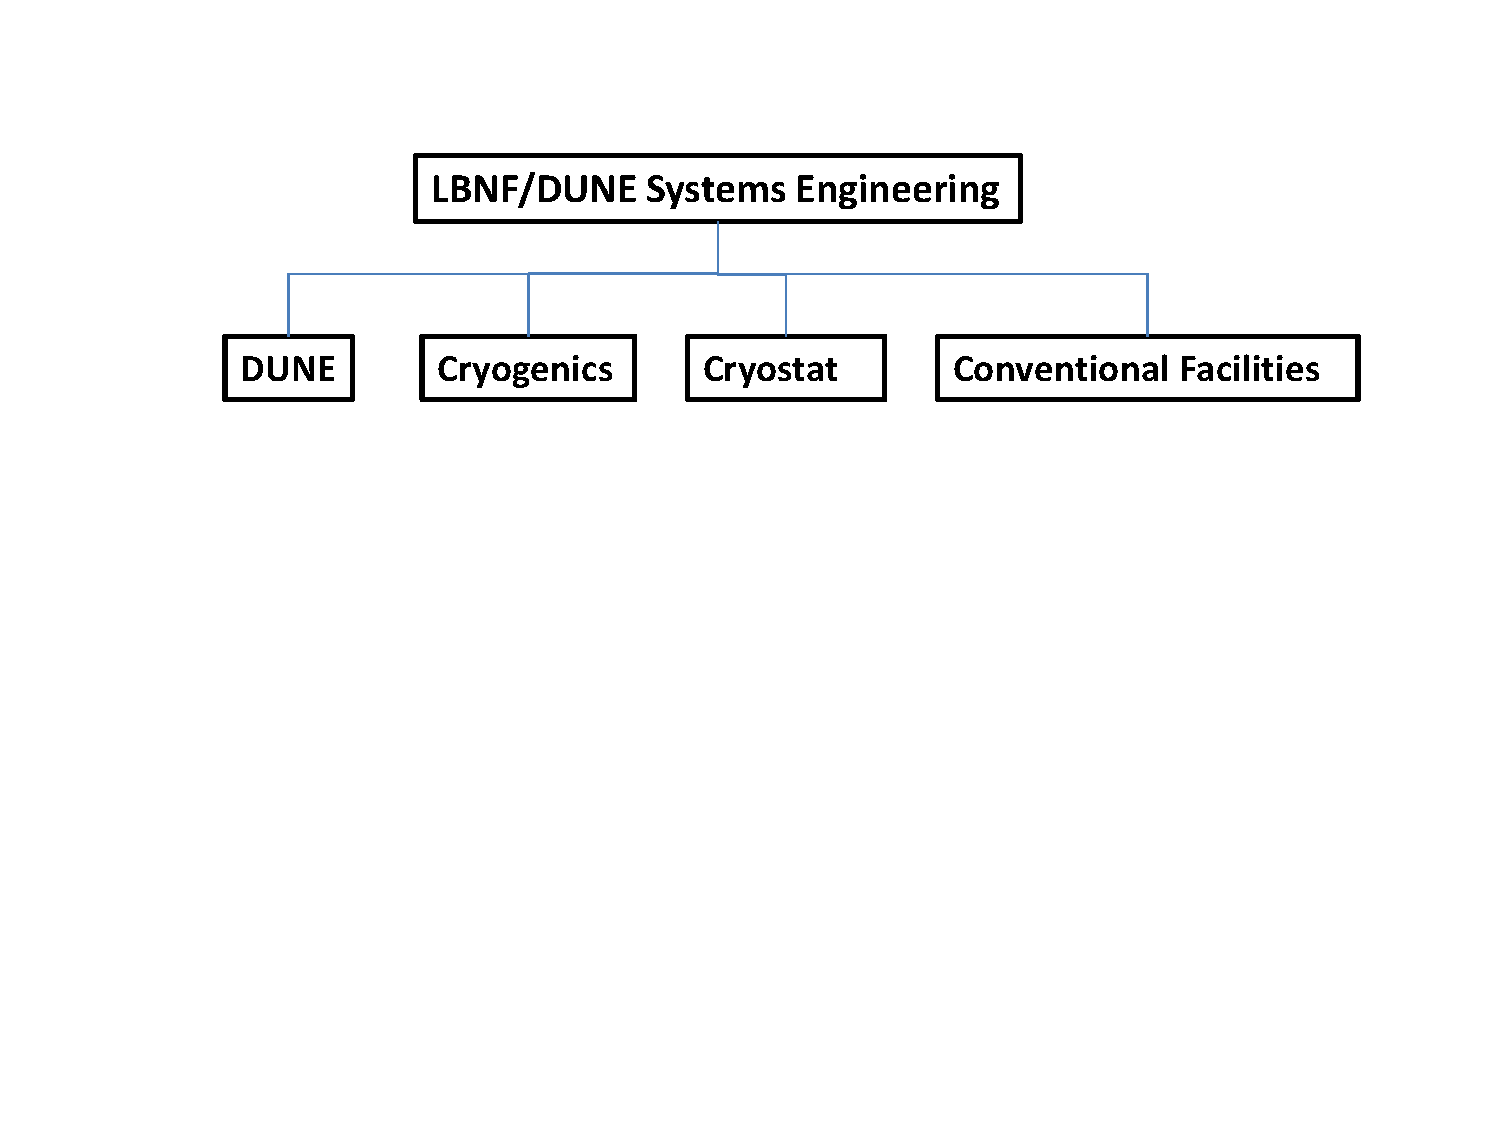
\includegraphics[width=\textwidth]{TC_SE_Org_Chart}
\end{dunefigure}

Proper integration of the \dwords{fd} within the supporting
facilities and infrastructure at \surf is a major engineering task.
The \dword{lbnf}/\dword{dune} Systems Engineer is responsible for the
interfaces between the major \dword{lbnf} and \dword{dune} systems
(conventional facilities, cryostats, cryogenics systems and
\dwords{detmodule}). The \dword{lbnf}/\dword{dune} systems engineering team
includes several engineers and designers with responsibility for
maintaining computer aided design (CAD) models. \Dword{dune} \dword{tc}
supports an engineering team that works directly with the
\dword{lbnf}/\dword{dune} systems engineering team to ensure that the
detector is properly integrated into the overall system.

\dword{tc} has been working with the \dword{lbnf}/\dword{dune} systems engineering team to
define requirements from \dword{dune} for the conventional facilities final
design for the detector chambers, \dword{cuc}, drifts
and utilities. \Dword{tc} is representing the interests of the \dword{dune} detector
in the conventional facilities (CF) design. This includes refining the
detector installation plan to understand how much space is needed in
front of the \dwords{tco} of the cryostats
and therefore of the size of the chambers. \dword{tc} continues to refine the
detector needs for utilities in the detector caverns and the \dword{cuc} 
where the \dword{daq} will be housed.

Physics requirements on \dword{tc} include cleanliness in the cryostats,
survey and alignment tolerances, and grounding and shielding
requirements. The cleanliness requirement is for ISO 8 (class
100,000), which will keep rates from dust radioactivity below those of
the inherent $^{39}$Ar background. The alignment tolerances are driven
by physics requirements on reconstructing tracks. Grounding and
shielding are critical to enable this very sensitive, low-noise
detector to achieve the required \dword{s/n}. The physics
requirements for \dword{lbnf} and \dword{dune} are maintained in
DocDB-112.
